\section{Auswertung}

\subsection{Temperaturverläufe}

Die aufgenommenen Messwerte befinden sich in Tabelle \ref{tab:temp}.
Es wird direkt jeweils ein Bar auf die abgelesenen Messwerte $p_a$ und $p_b$ addiert.
\begin{table}[H]
  \centering
  \caption{Temperaturverläufe}
  \label{tab:temp}
  \begin{tabular}{c S S S S c}
    \toprule
      {$t \:/\: \mathrm{s}$} & {$T_1 \:/\: \mathrm{°C}$} & {$T_2 \:/\: \mathrm{°C}$} &
      {$p_a \:/\: \mathrm{bar}$} & {$p_b \:/\: \mathrm{bar}$} & {$N \:/\: \mathrm{W}$}\\
    \midrule
    0  & 	20,1  &  19,6  & 	4,8  &  4,5  &  0  \\
    60  &  20,5  &  19,5  &  4,1  &  6,0  &  115  \\
    120  & 	21,5  &  19,1  &  		4,2  &  	6,0  &  	120  \\
    180  & 	22,6  &  18,0  &  		4,4  &  	6,1  &  	120  \\
    240  & 	23,7  &  17,1  &  		4,4  &  	7,0  &  	125  \\
    300  & 	24,9  &  16,1  &  		4,4  &  	7,0  &  	125  \\
    360  & 	26,1  &  15,2  &  		4,3  &  	7,0  &  	120  \\
    420  & 	27,3  &  14,4  &  		4,2  &  	7,0  &  	120  \\
    480  & 	28,5  &  13,7  &  		4,1  &  	7,5  &  	120  \\
    540  & 	29,5  &  13,0  &  		4,0  &  	7,5  &  	120  \\
    600  & 	30,7  &  12,3  &  		3,9  &  	8,0  &  	120  \\
    660  & 	31,7  &  11,6  &  		3,8  &  	8,0  &  	120  \\
    720  & 	32,7  &  10,9  &  		3,8  &  	8,0  &  	120  \\
    780  & 	33,7  &  10,2  &  		3,7  &  	8,5  &  	120  \\
    840  & 	34,6  &  9,5	  &  	3,6	  &  8,8	  &  120  \\
    900  & 	35,6  &  8,8	  &  	3,6	  &  9,0	  &  120  \\
    960  & 	36,4  &  8,2	  &  	3,6	  &  9,0	  &  120  \\
    1020  &  37,3  &  7,6  &  3,5  &  9,0	  &  120  \\
    1080  &  38,2  &  7,0  &  3,4  &  9,5	  &  120  \\
    1140  &  39,0  &  6,5  &  3,4  &  9,5	  &  120  \\
    1200  &  39,7  &  6,0  &  3,4  &  10,0  &  	120  \\
    1260  &  40,5  &  5,5  &  3,4  &  10,0  &  	120  \\
    1320  &  41,3  &  5,0  &  3,3  &  10,0  &  	125  \\
    1380  &  42,0  &  4,6  &  3,3  &  10,0  &  	125  \\
    1440  &  42,7  &  4,2  &  3,2  &  10,5  &  	125  \\
    1500  &  43,3  &  3,8  &  3,2  &  10,5  &  	125  \\
    1560  &  44,0  &  3,5  &  3,2  &  11,0  &  	125  \\
    1620  &  44,7  &  3,1  &  3,2  &  11,0  &  	125  \\
    1680  &  45,3  &  2,8  &  3,2  &  11,0  &  	125  \\
    1740  &  45,9  &  2,5  &  3,2  &  11,0  &  	115  \\
    1800  &  46,5  &  2,2  &  3,2  &  11,5  &  	115  \\
    1860  &  47,1  &  1,9  &  3,2  &  11,5  &  	115  \\
    1920  &  47,7  &  1,7  &  3,2  &  11,5  &  	115  \\
    1980  &  48,2  &  1,4  &  3,1  &  12,0  &  	115  \\
    2040  &  48,8  &  1,2  &  3,1  &  12,0  &  	115  \\
    2100  &  49,3  &  1,0  &  3,1  &  12,0  &  	115  \\
    2160  &  49,8  &  0,9  &  3,1  &  12,0  &  	115  \\
    \bottomrule
  \end{tabular}
\end{table}

Aus diesen Messwerten folgt Abbildung \ref{fig:temp}:
\begin{figure}[H]
  \centering
  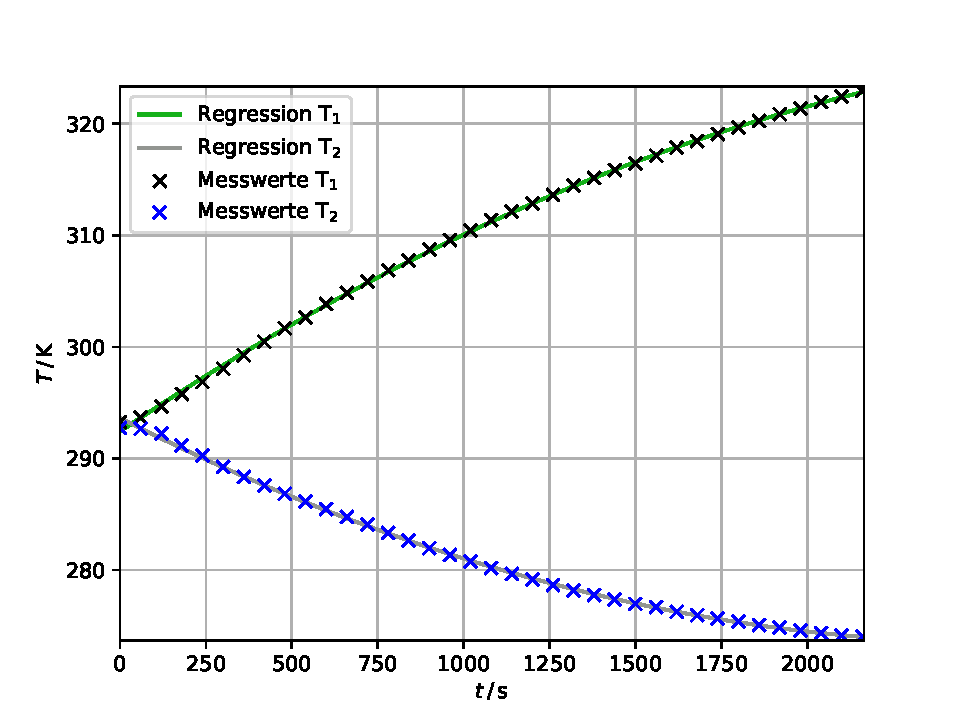
\includegraphics[width=\textwidth]{Plots/temp.pdf}
  \caption{$T$-$t$-Diagramm}
  \label{fig:temp}
\end{figure}

Mithilfe der Messwerte wird eine Regression $T(t) = a t^2 + b t + c$ durchgeführt, die für $T_1$ die Werte
\begin{align*}
  a &= \SI{-3,0728(897)e-6}{\kelvin \per \square \second} \\
  b &= \SI{0,0207(2)}{\kelvin \per \second} \\
  c &= \SI{292,4180(936)}{\kelvin}
\end{align*}

und für $T_2$ die Werte
\begin{align*}
  a &= \SI{3,0223(851)e-6}{\kelvin \per \square \second} \\
  b &= \SI{-0,0156(2)}{\kelvin \per \second} \\
  c &= \SI{293.6103(888)}{\kelvin}
\end{align*}

liefert.

\subsection{Güteziffer \label{sec:gut}}

Zunächst werden mithilfe von
\begin{equation*}
  \frac{\symup{d}T(t)}{\symup{d}t} = 2 a x + b
\end{equation*}

die Differenzenquotienten $\sfrac{\symup{d}T_1}{\symup{d}t}$
und $\sfrac{\symup{d}T_2}{\symup{d}t}$ für vier verschiedene Zeiten bestimmt.
Die Ergebnisse befinden sich in Tabelle \ref{tab:diff}.
\begin{table}[H]
  \centering
  \caption{Bestimmung der Differenzenquotienten}
  \label{tab:diff}
  \begin{tabular}{c S c S c}
    \toprule
      {$t \:/\: \mathrm{s}$} & {$T_1 \:/\: \mathrm{K}$} &
      {$\frac{\symup{d}T_1}{\symup{d}t} \:/\: \mathrm{\frac{K}{s}}$} &
      {$T_2 \:/\: \mathrm{K}$} &
      {$\frac{\symup{d}T_2}{\symup{d}t} \:/\: \mathrm{\frac{K}{s}}$} \\
    \midrule
    180  & 	295,75   & 0,0196 \pm 0,0002 &  291,15  & -0,0145 \pm 0,0002 \\
    600  & 	303,85   & 0,0170 \pm 0,0002 &  285,45  & -0,0120 \pm 0,0002 \\
    1020  &  310,45  & 0,0144 \pm 0,0003 &  280,75  & -0,0094 \pm 0,0003 \\
    1560  &  317,15  & 0,0111 \pm 0,0003 &  276,65  & -0,0062 \pm 0,0003 \\
    \bottomrule
  \end{tabular}
\end{table}

Die Fehler ergeben sich aus der Gauß'schen Fehlerfortpflanzung
\begin{equation}
  \delta = \sqrt{ \sum_{i=1}^{n}\left(\frac{\partial y}{\partial x_i} \Delta x_i\right)^2}.
  \label{eqn:gaus}
\end{equation}

Angewandt auf die Differenzenquotienten ergibt sich die Fehlerfortpflanzung
\begin{equation}
  \delta = \sqrt{(2t \cdot \Delta a)^2 + (1 \cdot \Delta b)^2}.
\end{equation}

Mithilfe von Gleichung \eqref{eqn:gut} und der in Tabelle \ref{tab:diff} berechneten Differenzenquotienten
lässt sich nun die Güteziffer $\nu$ für die vier augewählten Zeiten bestimmen.
Der Fehler ergibt sich aus der Gauß'schen Fehlerfortpflanzung
\begin{equation}
  \delta = \sqrt{\left(\frac{c_W m_W + m_K c_K}{N} \cdot \Delta \frac{\symup{d}T_1}{\symup{d}t}\right)^2}.
\end{equation}

Die Wärmekapazität des Reservoirs beträgt $\SI{750}{\joule \per \kelvin}$.
Die Wärmekapazität des Wassers ergibt sich mit der Wassermasse $m_W = \SI{4}{\kilo \gram}$ und der
spezifischen Wärmekapazität $c_W = \SI{4,182}{\kilo \joule \per \kilo \gram \kelvin}$ zu
\begin{equation*}
  c_W \cdot m_W = \SI{16728}{\joule \per \kelvin}.
\end{equation*}
Die Ergebnisse befinden sich in Tabelle \ref{tab:nu1}.
\begin{table}[H]
  \centering
  \caption{Bestimmung der Güteziffer aus den Messwerten für $T_1$}
  \label{tab:nu1}
  \begin{tabular}{c c S S}
    \toprule
      {$t \:/\: \mathrm{s}$} & {$\nu_{T_1}$} & {$\nu_\text{theo}$} &
      {Abweichung} \\
    \midrule
    180  & 2,86 \pm 0,05 &  64,29  & 95,56 \% \\
    600  & 2,48 \pm 0,05 &  16,51  & 84,98 \% \\
    1020 & 2,10 \pm 0,05 &  10,45  & 79,87 \% \\
    1560 & 1,56 \pm 0,05 &  7,83  & 80,13 \% \\
    \bottomrule
  \end{tabular}
\end{table}


\subsection{Massendurchsatz}

Zur Berechung des Massendurchsatzes $\sfrac{\symup{d} m}{\symup{d} t}$ wird zunächst die Verdampfungswärme $L$
mithilfe einer Dampfdruckkurve (s. Abbildung \ref{fig:dampf}) bestimmt. Der Umgebungsdruck $p_0$
beträgt $1 \, \mathrm{bar}$.
\begin{figure}[H]
  \centering
  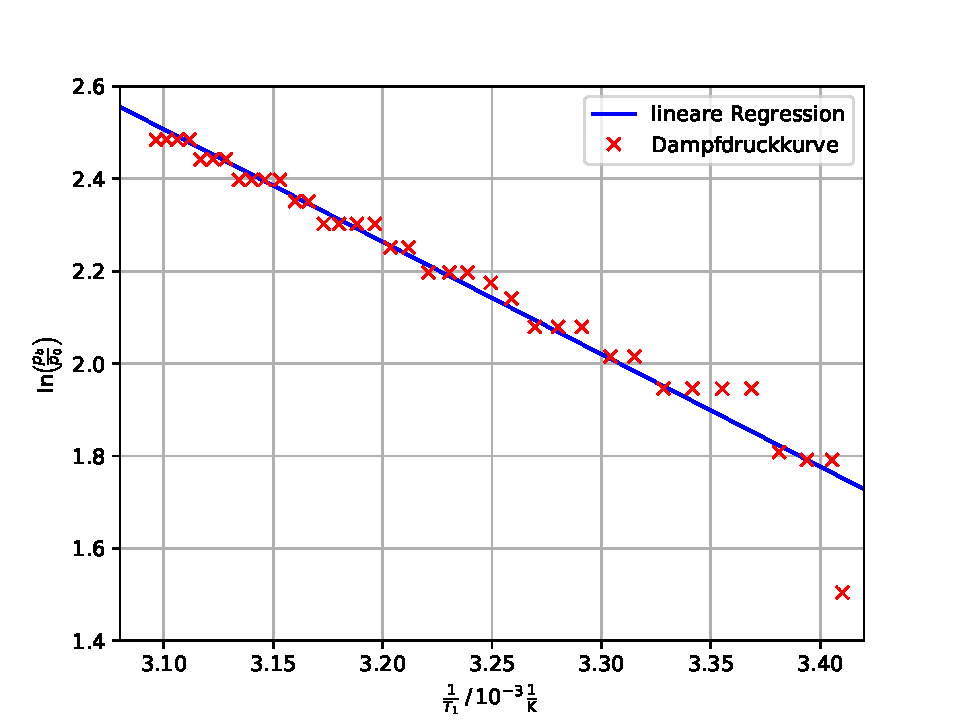
\includegraphics[width=\textwidth]{Plots/dampf.pdf}
  \caption{$\ln \left(\frac{p_b}{p_0}\right)$-$\frac{1}{T_1}$-Diagramm mit Dampfdruckkurve zur Bestimmung der Verdampfungswärme}
  \label{fig:dampf}
\end{figure}

Eine lineare Regression $f(x) = -d \cdot x + e$ liefert die Werte
\begin{align*}
  d &= \SI{2433,62(8530)}{\K} \\
  e &= 10,05 \pm 0,28 .
\end{align*}

Aus Gleichung \eqref{eqn:dampf} (s. \cite[5]{sample2}) und der Gauß'schen Fehlerfortpflanzung \eqref{blub}
\begin{equation}
  \delta = \sqrt{(d R \cdot \Delta d)^2}
  \label{blub}
\end{equation}

\begin{equation}
 \ln \left( \frac{p}{p_0} \right) = - \frac{L}{R} \cdot \frac{1}{T}
 \label{eqn:dampf}
\end{equation}

ergibt sich mit der allgemeinen Gaskonstanten $R$ die Verdampfungswärme
\begin{equation*}
  L = \SI{20233,10(70919)}{\joule \per \mol}.
\end{equation*}

Der Massendurchsatz errechnet sich aus Gleichung \eqref{eqn:masse}.
Die Ergebnisse mit ihren Fehlern nach Gleichung \eqref{eqn:blub} befinden sich in Tabelle \ref{tab:mas}.
\begin{equation}
    \delta = \sqrt{\left(-\frac{m_w c_w + m_k c_k}{L^2} \frac{\symup{d} T_2}{\symup{d} t}  \cdot \Delta L\right)^2 + \left(\frac{m_w c_w + m_k c_k}{L} \cdot \Delta \frac{\symup{d} T_2}{\symup{d} t}\right)^2}
    \label{eqn:blub}
\end{equation}

\begin{table}[H]
  \centering
  \caption{Massendurchsatz}
  \label{tab:mas}
  \begin{tabular}{c c c}
    \toprule
      {$t \:/\: \mathrm{s}$} & {$\frac{\symup{d} m}{\symup{d} t} \:/\: \frac{\mathrm{mol}}{\mathrm{s}}$} &
      {$\frac{\symup{d} m}{\symup{d} t} \:/\: \frac{\mathrm{g}}{\mathrm{s}}$} \\
    \midrule
    180  &  0,0125 \pm  0,0005 & 1,4426 \pm 0,0541  \\
    600  &  0,0104 \pm  0,0004 & 1,1904 \pm 0,0469  \\
    1020 &  0,0082 \pm  0,0004 & 0,9382 \pm 0,0417  \\
    1560 &  0,0053 \pm  0,0003 & 0,6139 \pm 0,0389  \\
    \bottomrule
  \end{tabular}
\end{table}

\subsection{Mechanische Kompressorleistung}
Mithilfe der idealen Gasgleichung \eqref{eqn:gas}
\begin{equation}
  p V = n R T \iff n R = \frac{p V}{T} = \text{const.}
  \label{eqn:gas}
\end{equation}

ergibt sich mit $\rho_0 = \SI{5514}{\gram \per \cubic \meter}$, $p_0 = 1 \, \mathrm{bar}$,
$\kappa = 1,14$ und $T_0 = 0 \, \mathrm{°C}$ die Dichte des Transportmediums im gasförmigen Zustand
\begin{equation}
  \rho = \frac{\rho_0 \cdot T_0 \cdot p_a}{T_2 \cdot p_0}.
\end{equation}

Eingesetzt in Gleichung \eqref{eqn:leist} erhält man
\begin{equation}
  N_\text{mech} = \frac{1}{\kappa - 1} \cdot \left(p_b \cdot \sqrt[\kappa]{\frac{p_a}{p_b}} - p_a \right) \cdot \frac{T_2 \cdot p_0}{\rho_0 \cdot T_0 \cdot p_a} \cdot \frac{\symup{d} m}{\symup{d} t}
\end{equation}

für die mechanische Kompressorleistung.
Die Ergebnisse mit ihren Fehlern nach Gleichung \eqref{eqn:bliblub} befinden sich in Tabelle \ref{tab:mech}
\begin{equation}
  \delta = \sqrt{\left(\frac{1}{\kappa - 1} \cdot \left(p_b \cdot \sqrt[\kappa]{\frac{p_a}{p_b}} - p_a \right) \cdot \frac{T_2 \cdot p_0}{\rho_0 \cdot T_0 \cdot p_a} \cdot \Delta \frac{\symup{d} m}{\symup{d} t} \right)^2}
  \label{eqn:bliblub}
\end{equation}

\begin{table}[H]
  \centering
  \caption{mechanische Kompressorleistung}
  \label{tab:mech}
  \begin{tabular}{c c c}
    \toprule
      {$t \:/\: \mathrm{s}$} & {$N_\text{mech} \:/\: \mathrm{W}$} &
      {Wirkungsgrad} \\
    \midrule
    180  & 8,16 \pm  0,31 & 6,8 \%  \\
    600  & 14,88 \pm  0,59 & 12,4 \%  \\
    1020 & 15,37 \pm  0,68 & 12,8 \%  \\
    1560 & 13,20 \pm  0,84 & 10,6 \%  \\
    \bottomrule
  \end{tabular}
\end{table}
